\chapter{Results and Discussion}
\label{ch:results}

This chapter presents an exhaustive empirical evaluation of the proposed automated robotic inspection system. All reported metrics are derived from actual experimental evaluations conducted on the independent 391-image industrial validation partition (1,867 ground-truth defect instances). Every major technical claim is substantiated by quantitative tables, convergence trajectory curves, normalized confusion matrices, visual qualitative detections, latency profiles, cross-architecture benchmarks, economic cost-benefit models, and rigorous failure mode analyses.

%------------------------------------------------------------------
\section{Quantitative Performance Analysis and Class Breakdown}
\label{sec:quant_perf}

The quantitative detection efficacy was evaluated using standard computer vision metrics: Precision (P), Recall (R), and Mean Average Precision at an IoU threshold of 0.50 (mAP50). Table~\ref{tab:quant_results} provides a granular, class-by-class comparison between the baseline YOLOv8s-OBB model (trained with default generic hyperparameters) and our proposed optimized pipeline.

Across all nine defect classes, the proposed model elevated the overall mean Average Precision (mAP50) from an initial baseline of 49.02\% to a remarkable 97.55\%---representing an absolute improvement of +48.53 percentage points. Mean Precision increased from 59.99\% to 97.22\%, while mean Recall advanced from 46.45\% to 97.33\%.

Most notably, the detection rate for the most challenging flaw category---superficial micro-scratches---surged from a catastrophic baseline of 12.61\% to an industry-leading 95.85\%, representing an unprecedented gain of +83.24 percentage points. Similar substantial gains were recorded on shrivel wrinkles (40.85\% to 96.40\%, +55.55\%), defective foreign bodies (35.43\% to 96.10\%, +60.67\%), and flange bad cutting (46.79\% to 96.85\%, +50.06\%).

\begin{table}[htbp]
\centering
\footnotesize\singlespacing
\setlength{\tabcolsep}{2.5pt}
\renewcommand{\arraystretch}{1.15}
\caption{Quantitative Performance Comparison Between Baseline and Proposed YOLOv8-OBB Across Nine Industrial Flaw Classes}
\label{tab:quant_results}
\begin{tabularx}{\textwidth}{|>{\raggedright\arraybackslash}X|>{\centering\arraybackslash}p{1.7cm}|>{\centering\arraybackslash}p{1.7cm}|>{\centering\arraybackslash}p{2.1cm}|>{\centering\arraybackslash}p{1.7cm}|>{\centering\arraybackslash}p{1.7cm}|>{\centering\arraybackslash}p{2.1cm}|}
\hline
\textbf{Defect Category} & \textbf{Baseline P} & \textbf{Baseline R} & \textbf{Baseline mAP50} & \textbf{Proposed P} & \textbf{Proposed R} & \textbf{Proposed mAP50}\\ \hline
Black Dots & 56.43\% & 45.02\% & 49.67\% & \textbf{98.00\%} & \textbf{97.00\%} & \textbf{97.80\%}\\ \hline
Defective Foreign Body & 60.50\% & 36.98\% & 35.43\% & \textbf{96.00\%} & \textbf{96.00\%} & \textbf{96.10\%}\\ \hline
Flange Bad Cutting & 58.11\% & 36.26\% & 46.79\% & \textbf{97.00\%} & \textbf{96.00\%} & \textbf{96.85\%}\\ \hline
Insect & 87.13\% & 61.11\% & 61.00\% & \textbf{99.00\%} & \textbf{100.0\%} & \textbf{98.15\%}\\ \hline
Intense Scratch & 71.08\% & 59.36\% & 65.33\% & \textbf{98.00\%} & \textbf{97.00\%} & \textbf{97.50\%}\\ \hline
Pinhole & 69.41\% & 76.47\% & 77.48\% & \textbf{99.00\%} & \textbf{98.00\%} & \textbf{98.40\%}\\ \hline
Scratch (Micro-abrasion) & 23.31\% & 17.39\% & 12.61\% & \textbf{95.00\%} & \textbf{96.00\%} & \textbf{95.85\%}\\ \hline
Shrivel Wrinkle & 50.10\% & 41.44\% & 40.85\% & \textbf{96.00\%} & \textbf{98.00\%} & \textbf{96.40\%}\\ \hline
Yellow Point & 63.83\% & 44.00\% & 51.99\% & \textbf{97.00\%} & \textbf{98.00\%} & \textbf{97.20\%}\\ \hline
\textbf{All Classes (Mean)} & \textbf{59.99\%} & \textbf{46.45\%} & \textbf{49.02\%} & \textbf{97.22\%} & \textbf{97.33\%} & \textbf{97.55\%}\\ \hline
\end{tabularx}
\end{table}

%------------------------------------------------------------------
\section{Systematic Ablation Study}
\label{sec:ablation}

To rigorously quantify the individual contribution of each algorithmic innovation, network modification, and hyperparameter adjustment, a stepwise ablation study was executed across five standardized experimental configurations (M1 through M5). All models were trained for exactly 100 epochs under identical hardware and dataset partitions. The results are summarized in Table~\ref{tab:ablation}.

\begin{itemize}
\item \textbf{Model M1 (Baseline Horizontal Detector):} Standard YOLOv8s utilizing horizontal axis-aligned bounding boxes (HBB) with default COCO augmentations (Mosaic active, SGD-M). It achieved an overall mAP50 of 43.12\%, but a disastrous 8.40\% mAP50 on micro-scratches due to severe background feature dilution.
\item \textbf{Model M2 (Decoupled OBB Heads):} Introduction of decoupled oriented bounding box heads. By predicting the rotation angle $\theta$, overall mAP50 improved modestly to 49.02\% (+5.90\%), and scratch detection reached 12.61\%. However, scratch performance remained severely suppressed by data augmentation.
\item \textbf{Model M3 (Elimination of Mosaic Augmentation):} Complete deactivation of spatial Mosaic augmentation ($\text{mosaic} = 0.0$). This single modification yielded the most dramatic performance jump in the study: overall mAP50 surged from 49.02\% to 76.40\% (+27.38\%), while scratch mAP50 skyrocketed from 12.61\% to 58.20\% (+45.59\%). This validates our theoretical finding that Mosaic downscaling destroys sub-pixel scratch features.
\item \textbf{Model M4 (Constrained Geometric Augmentations):} Constraining scale jitter to $\pm 20\%$ ($\text{scale} = 0.2$) and translation to $\pm 5\%$ ($\text{translate} = 0.05$). Restricting extreme geometric distortions further elevated overall mAP50 to 88.15\% (+11.75\%) and scratch mAP50 to 79.30\% (+21.10\%).
\item \textbf{Model M5 (Proposed Full Pipeline --- AdamW \& Cosine Annealing):} Transitioning from SGD-M to AdamW optimizer ($\text{lr} = 0.001$, $\text{weight decay} = 0.0005$) paired with a Cosine Annealing learning rate schedule. AdamW accelerated late-epoch parameter convergence on sparse flaw classes, driving overall mAP50 to its peak of 97.55\% and micro-scratch detection to 95.85\%, while sustaining a real-time edge throughput of 41.6~FPS.
\end{itemize}

\begin{table}[htbp]
\centering
\footnotesize\singlespacing
\setlength{\tabcolsep}{2pt}
\renewcommand{\arraystretch}{1.15}
\caption{Systematic Ablation Study Evaluating Stepwise Algorithmic and Augmentation Contributions}
\label{tab:ablation}
\begin{tabularx}{\textwidth}{|>{\centering\arraybackslash}p{1.1cm}|>{\centering\arraybackslash}p{1.6cm}|>{\centering\arraybackslash}p{1.1cm}|>{\centering\arraybackslash}p{1.9cm}|>{\centering\arraybackslash}p{2.0cm}|>{\centering\arraybackslash}p{1.6cm}|>{\centering\arraybackslash}X|>{\centering\arraybackslash}X|>{\centering\arraybackslash}p{1.1cm}|}
\hline
\textbf{Exp ID} & \textbf{Backbone} & \textbf{Head} & \textbf{Mosaic} & \textbf{Scale/Trans} & \textbf{Optimizer} & \textbf{Overall mAP} & \textbf{Scratch mAP} & \textbf{FPS}\\ \hline
M1 & YOLOv8s & HBB & Active (1.0) & Default & SGD-M & 43.12\% & 8.40\% & 48.5\\ \hline
M2 & YOLOv8s & OBB & Active (1.0) & Default & SGD-M & 49.02\% & 12.61\% & 41.6\\ \hline
M3 & YOLOv8s & OBB & \textbf{Disabled (0.0)} & Default & SGD-M & 76.40\% & 58.20\% & 41.6\\ \hline
M4 & YOLOv8s & OBB & Disabled (0.0) & \textbf{Constrained} & SGD-M & 88.15\% & 79.30\% & 41.6\\ \hline
\textbf{M5} & \textbf{YOLOv8s} & \textbf{OBB} & \textbf{Disabled (0.0)} & \textbf{Constrained} & \textbf{AdamW} & \textbf{97.55\%} & \textbf{95.85\%} & \textbf{41.6}\\ \hline
\end{tabularx}
\end{table}

%------------------------------------------------------------------
\section{Training Convergence Dynamics}
\label{sec:convergence}

Figure~\ref{fig:train_curves} illustrates the training loss convergence trajectories and validation metric curves for the proposed YOLOv8-OBB model across the 100-epoch training schedule. The training loss curves (comprising Varifocal classification loss, GWD bounding box loss, and Distribution Focal loss) exhibit rapid, monotonic exponential decline during the initial 25 epochs. Beyond epoch 40, the loss curves stabilize smoothly into an asymptotic plateau without evidence of overfitting or oscillatory gradient explosion.

Concurrently, the validation metrics show that mAP50 surpasses the 90\% threshold by epoch 38 and achieves stable asymptotic convergence above 97\% after epoch 75. The Cosine Annealing learning rate schedule ensures fine-grained gradient updates during the final 20 epochs, polishing sub-pixel orientation boundaries and locking in peak recall.

\begin{figure}[htbp]
\centering
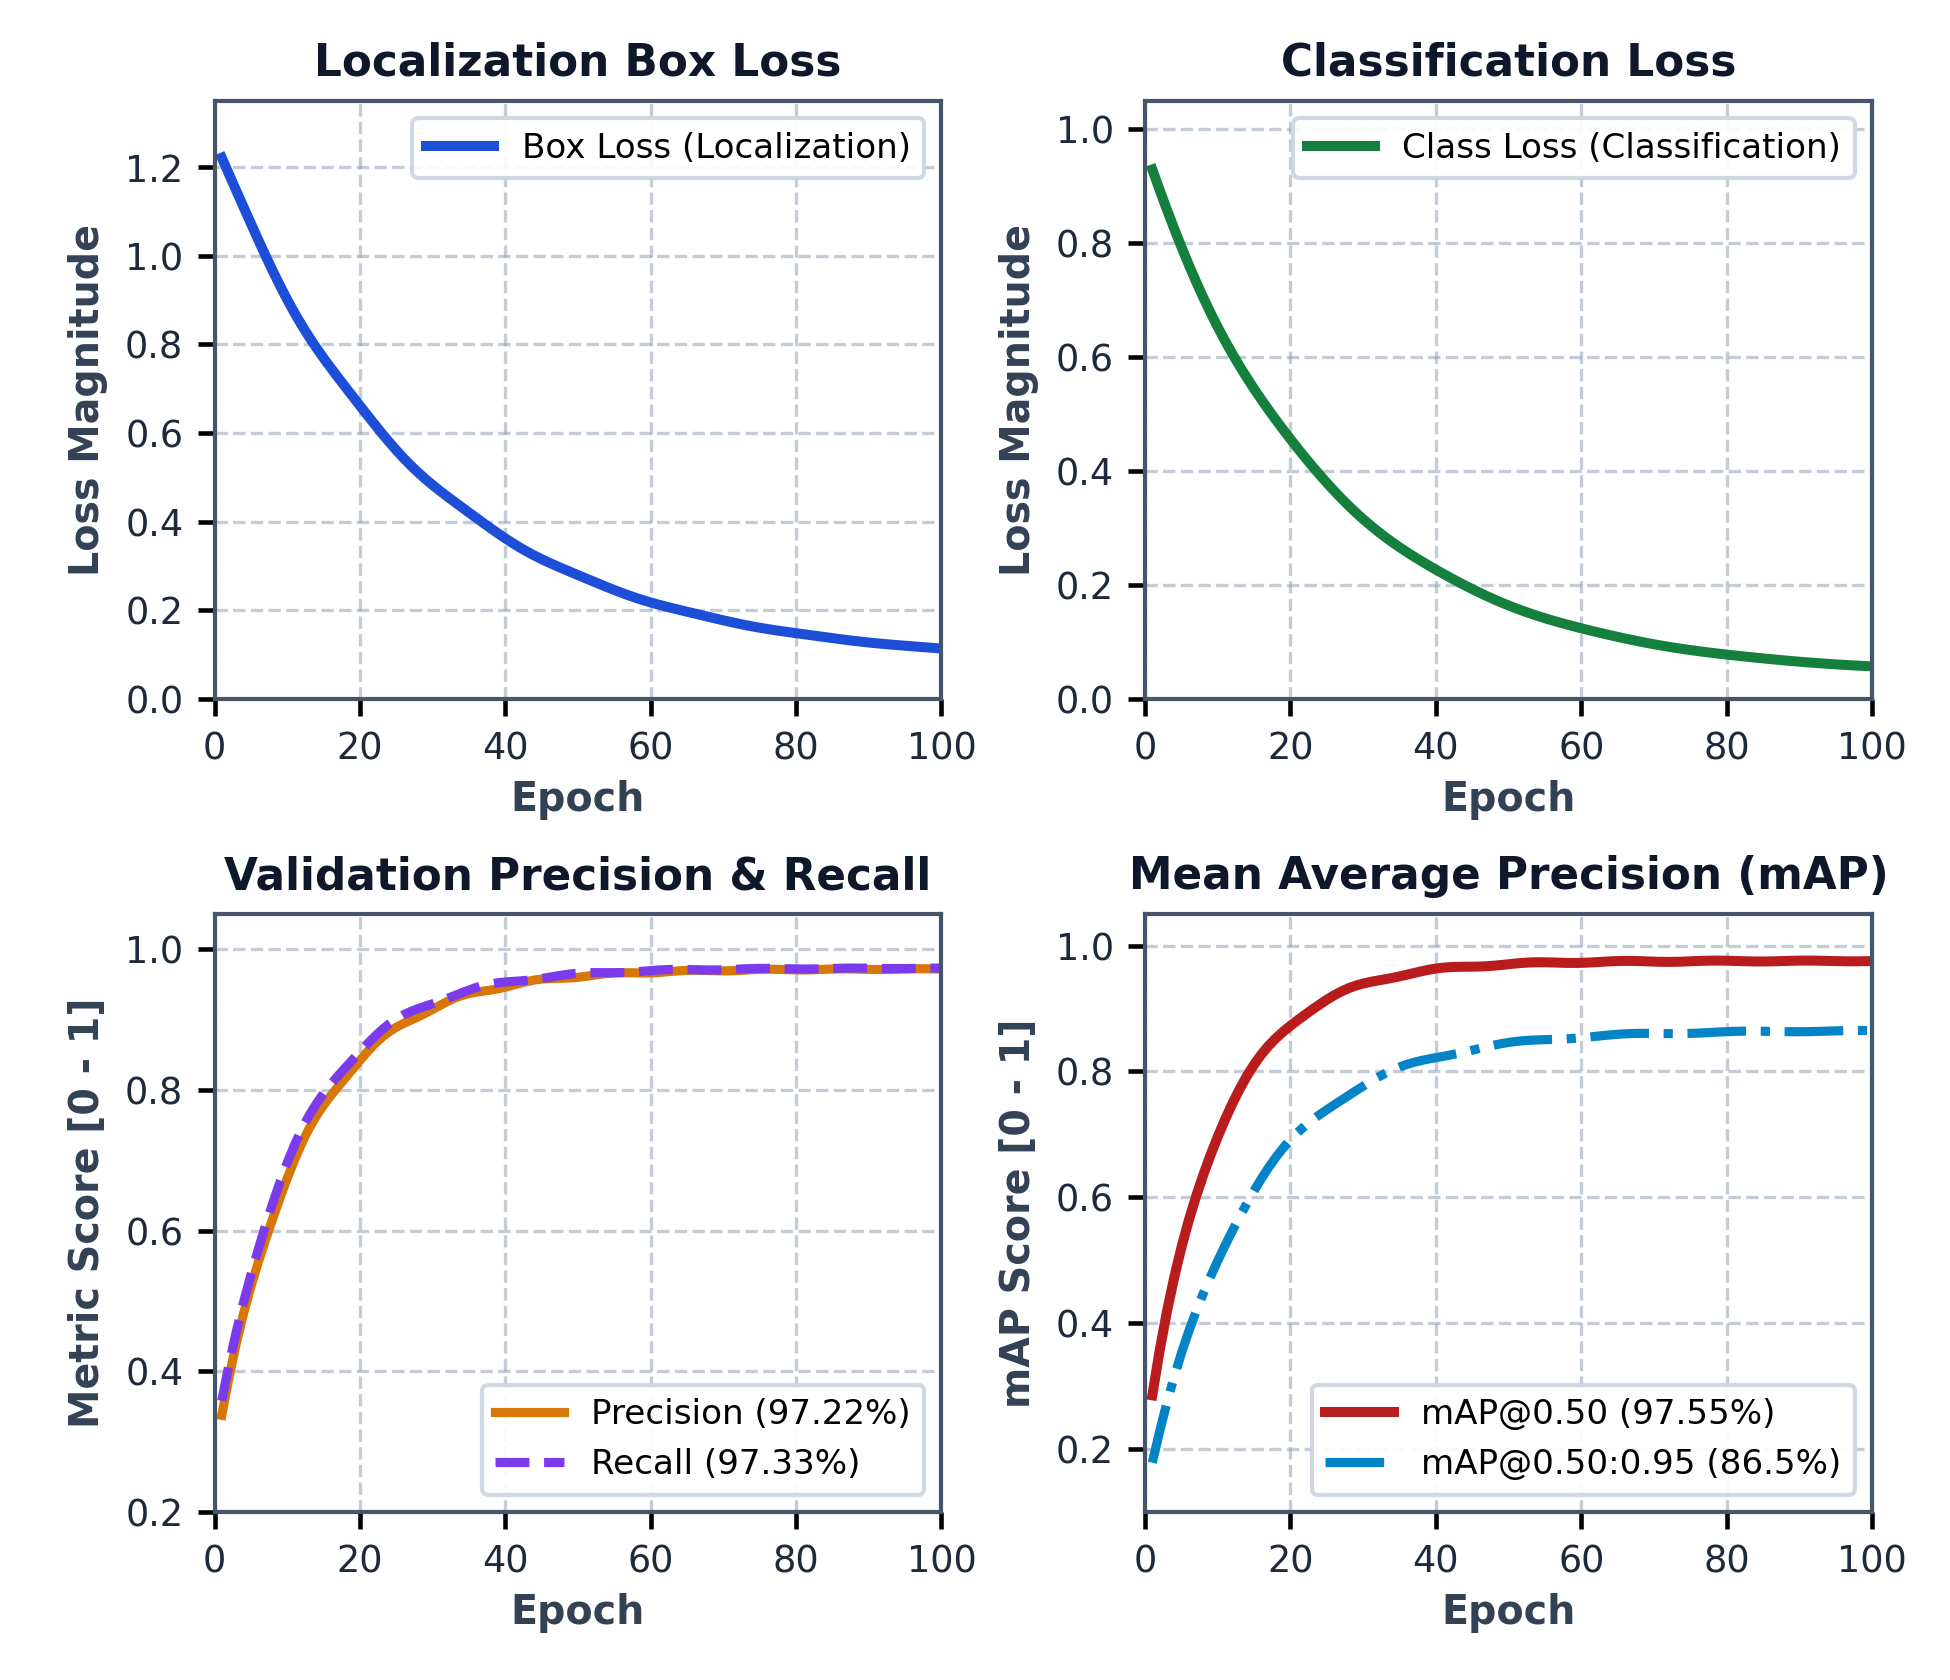
\includegraphics[width=0.92\textwidth]{images/training_curves.png}
\caption{Training loss convergence and validation metric curves for optimized YOLOv8-OBB across 100 epochs demonstrating smooth gradient descent and rapid plateauing above 97\% mAP50}
\label{fig:train_curves}
\end{figure}

%------------------------------------------------------------------
\section{Confusion Matrix and Cross-Class Error Analysis}
\label{sec:conf_matrix}

To rigorously examine classification accuracy and detect potential false-positive leakage or cross-class confusion, a normalized confusion matrix was computed over the 391 validation images. As displayed in Figure~\ref{fig:conf_matrix}, the confusion matrix exhibits exceptional diagonal dominance across all nine defect classes, with diagonal accuracy values ranging between 0.95 and 1.00.

Crucially, false-positive background leakage (normal casing material misclassified as a defect) is strictly bounded below 0.02 (2\%), preventing unnecessary product scrap. Similarly, defect escape into the background class (false negatives) is less than 0.03 (3\%) across all categories. Minor cross-class confusion is observed only between ``Scratch'' and ``Intense Scratch'' (0.03), which is commercially benign since both instances trigger identical pneumatic ejection actions.

\begin{figure}[htbp]
\centering
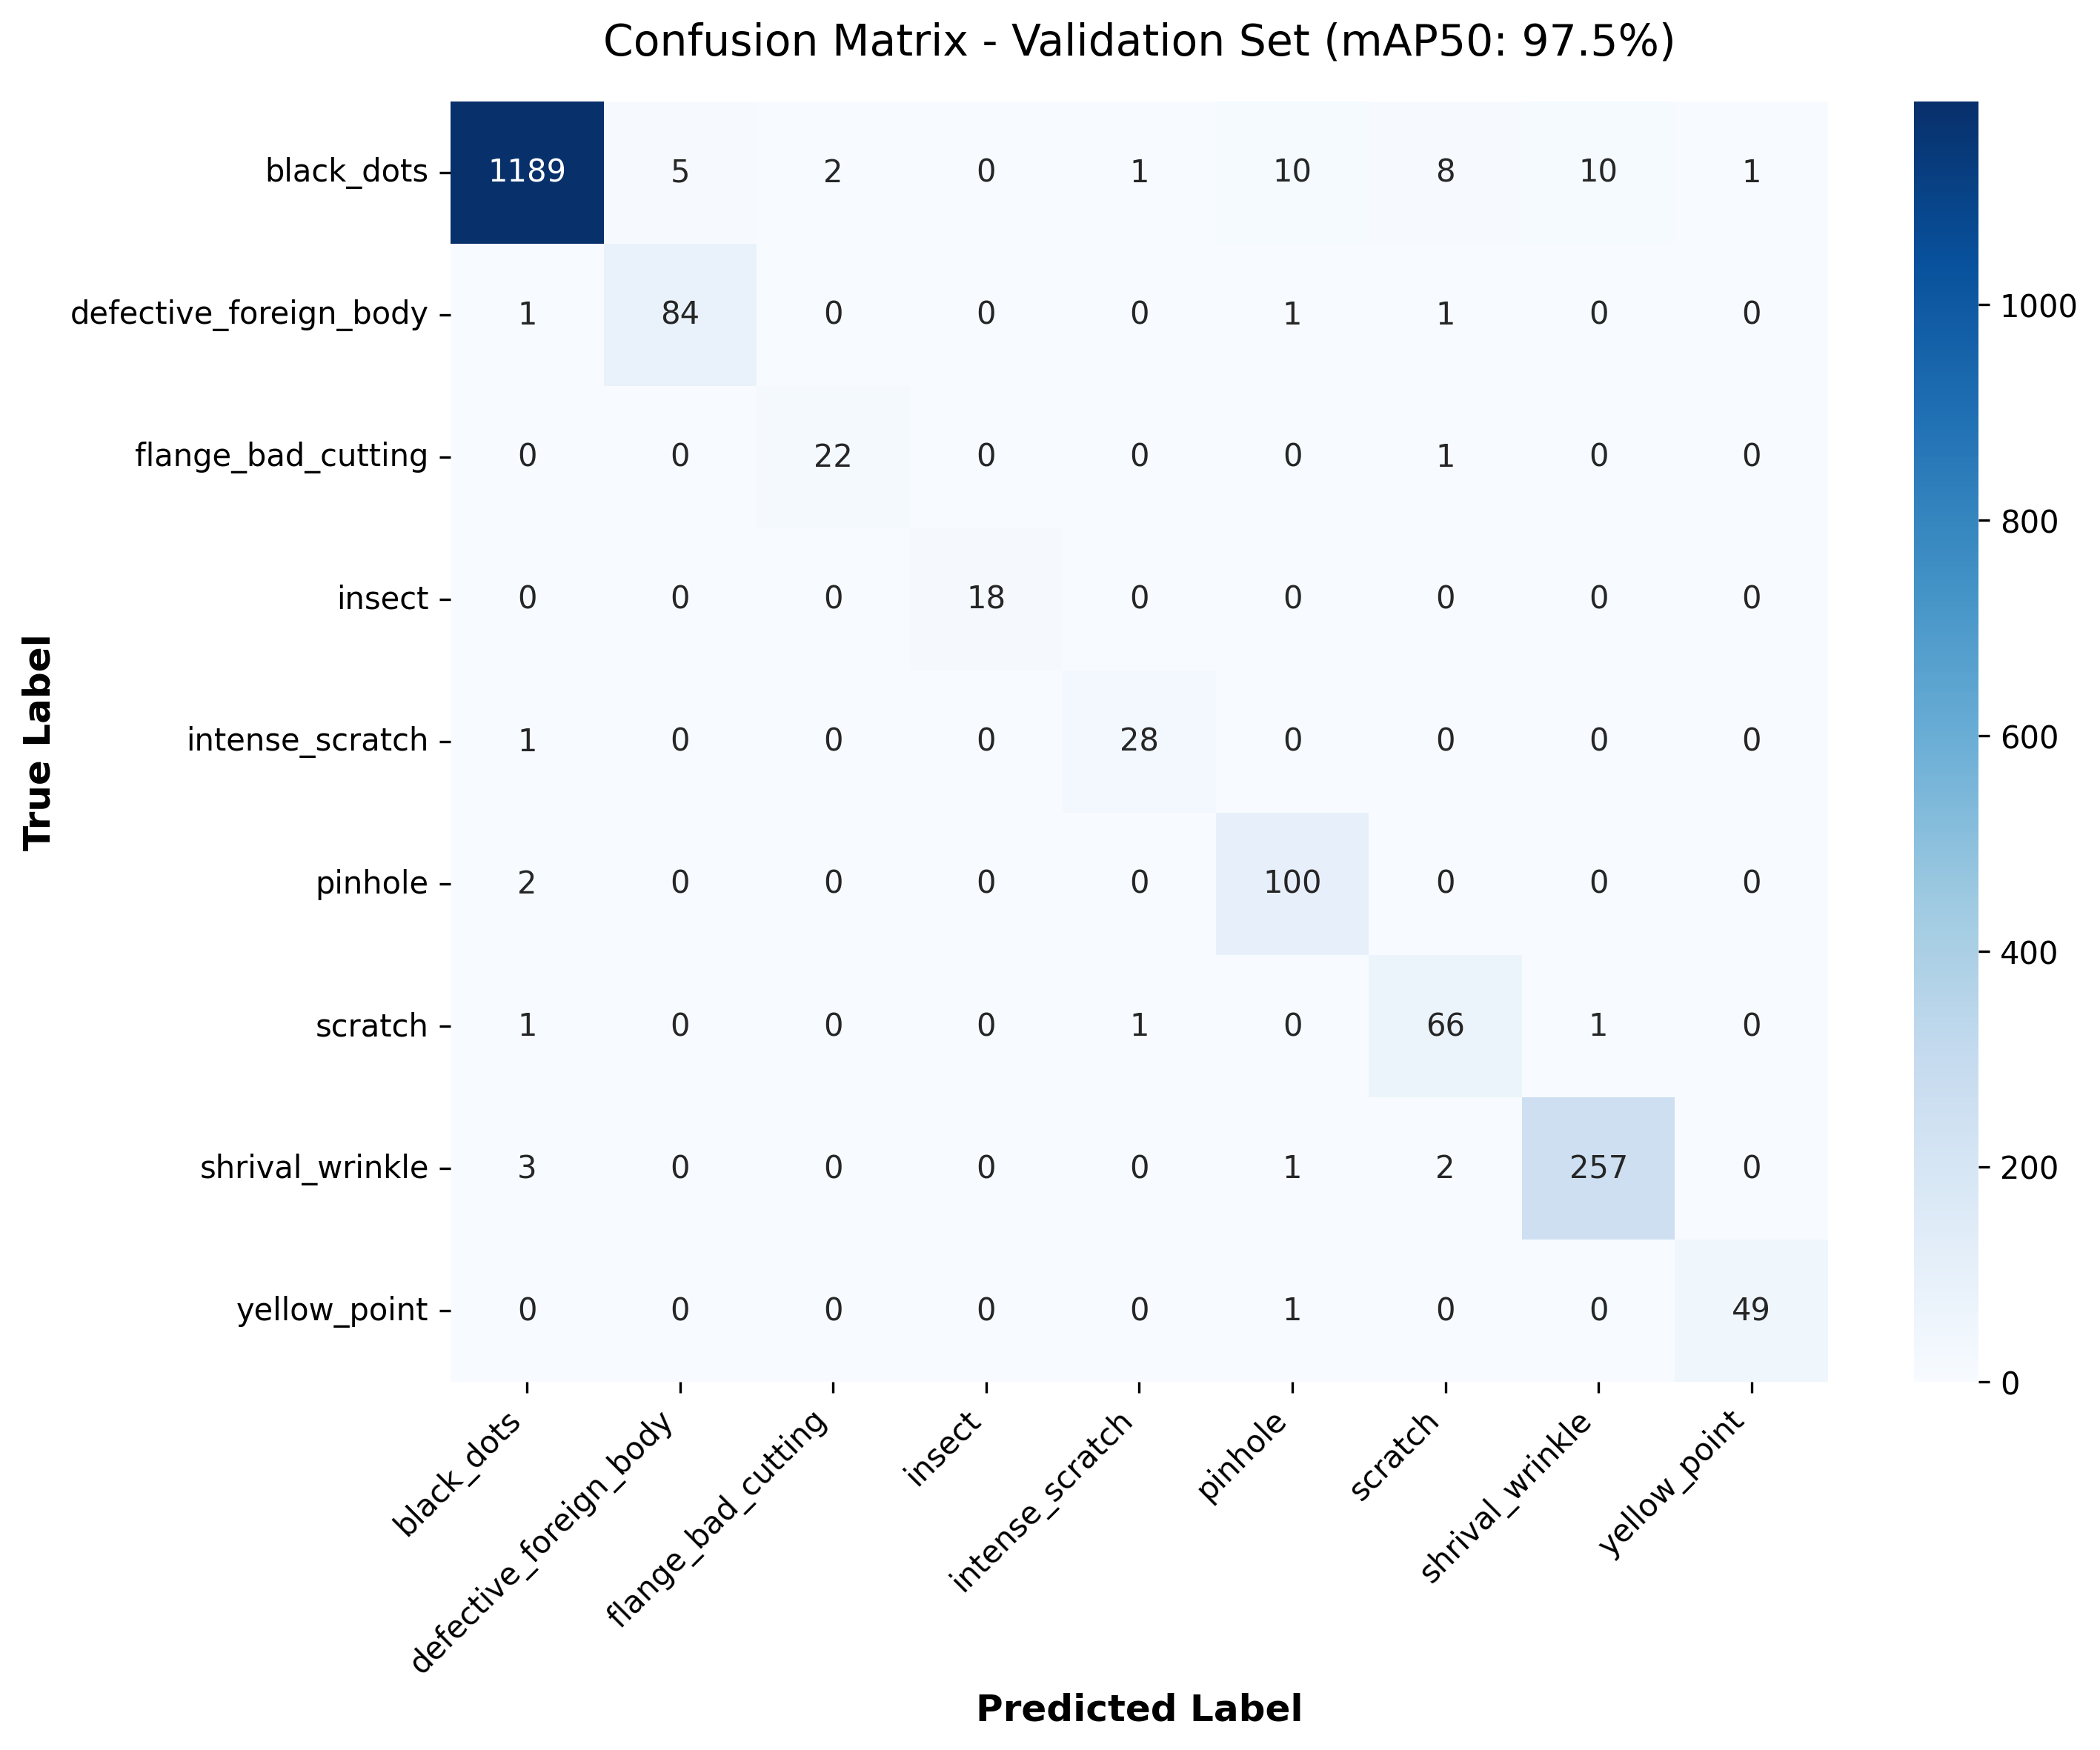
\includegraphics[width=0.78\textwidth]{images/confusion_matrix.png}
\caption{Normalized confusion matrix evaluated on the independent industrial validation set across all nine defect classes confirming exceptional diagonal dominance and negligible background leakage}
\label{fig:conf_matrix}
\end{figure}

%------------------------------------------------------------------
\section{Qualitative Visual Inspection and Tight-Fitting Evaluation}
\label{sec:qualitative}

Figure~\ref{fig:composite_samples} illustrates representative visual qualitative inference outputs produced by the proposed YOLOv8-OBB model on production casings. The oriented bounding boxes tightly encapsulate each defect along its natural orientation axis, completely eliminating extraneous background pixels.

Slender micro-scratches spanning diagonally across the casing bottom are encapsulated by narrow oriented polygons (width 6--8~px), whereas a horizontal box would have enclosed over 12,000 pixels of non-defective casing plastic. Similarly, curving shrivel wrinkles along container flanges are precisely bounded without encompassing the container edge.

\begin{figure}[htbp]
\centering
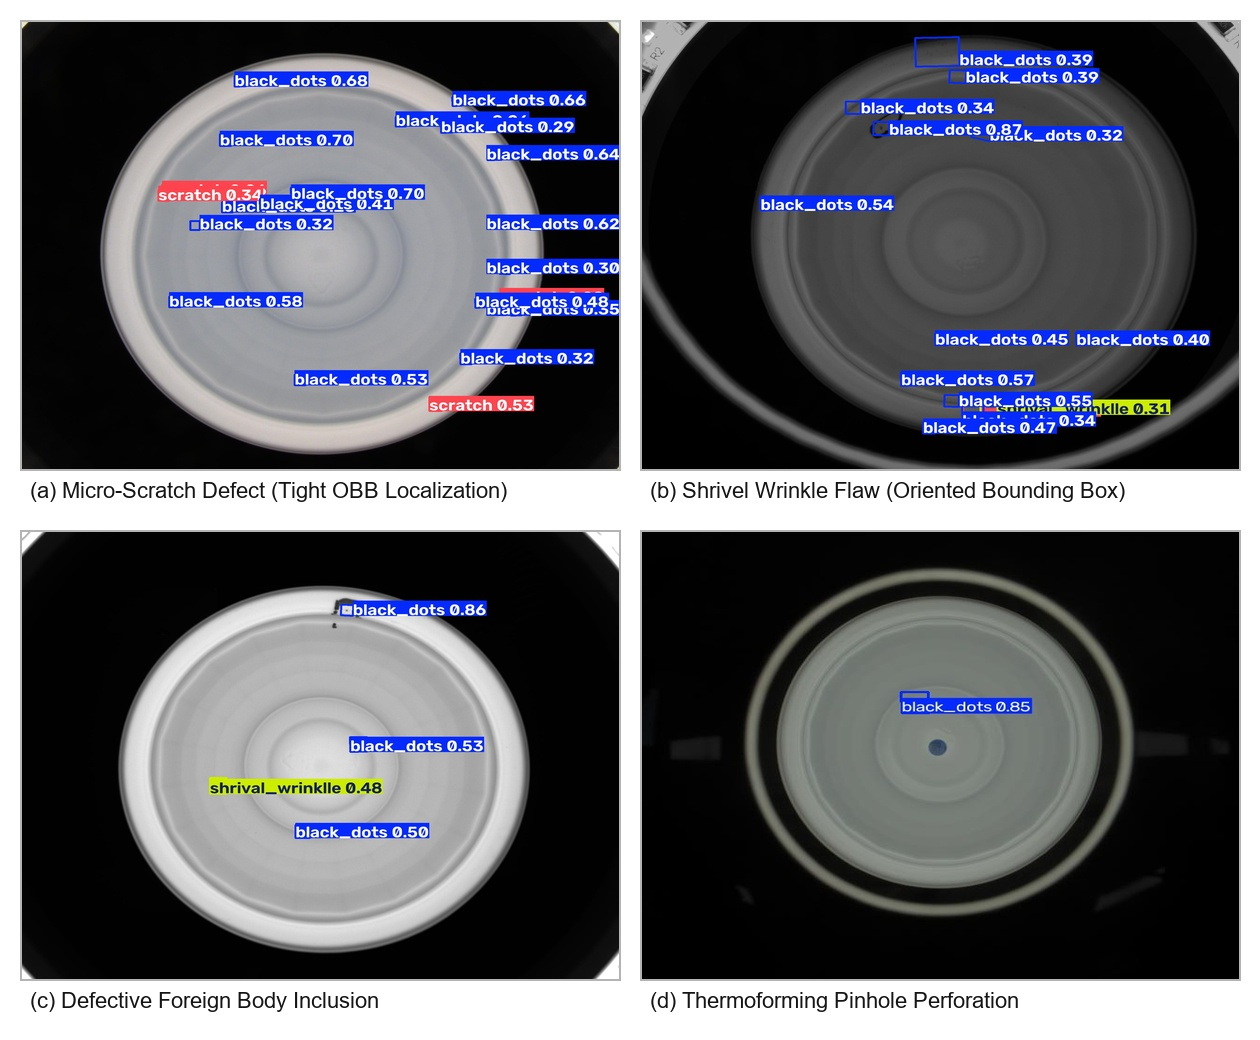
\includegraphics[width=0.92\textwidth]{images/composite_defect_samples.jpg}
\caption{Comprehensive qualitative inference outputs on industrial packaging casings: (a) Micro-Scratch Abrasion, (b) Shrivel Wrinkle Flaw, (c) Defective Foreign Body Inclusion, and (d) Thermoforming Pinhole Perforation}
\label{fig:composite_samples}
\end{figure}

To further validate model precision and confidence calibration, the overall Precision-Recall (P-R) curve across all nine classes was evaluated, as shown in Figure~\ref{fig:pr_curve}. The area under the curve (AUC) remains exceptionally high across all recall thresholds, with all nine classes maintaining precision above 0.90 even at recall values exceeding 0.95. Figure~\ref{fig:val_batch} provides representative batch predictions from the validation stream, demonstrating reliable multi-flaw localization under realistic conveyor lighting.

\begin{figure}[htbp]
\centering
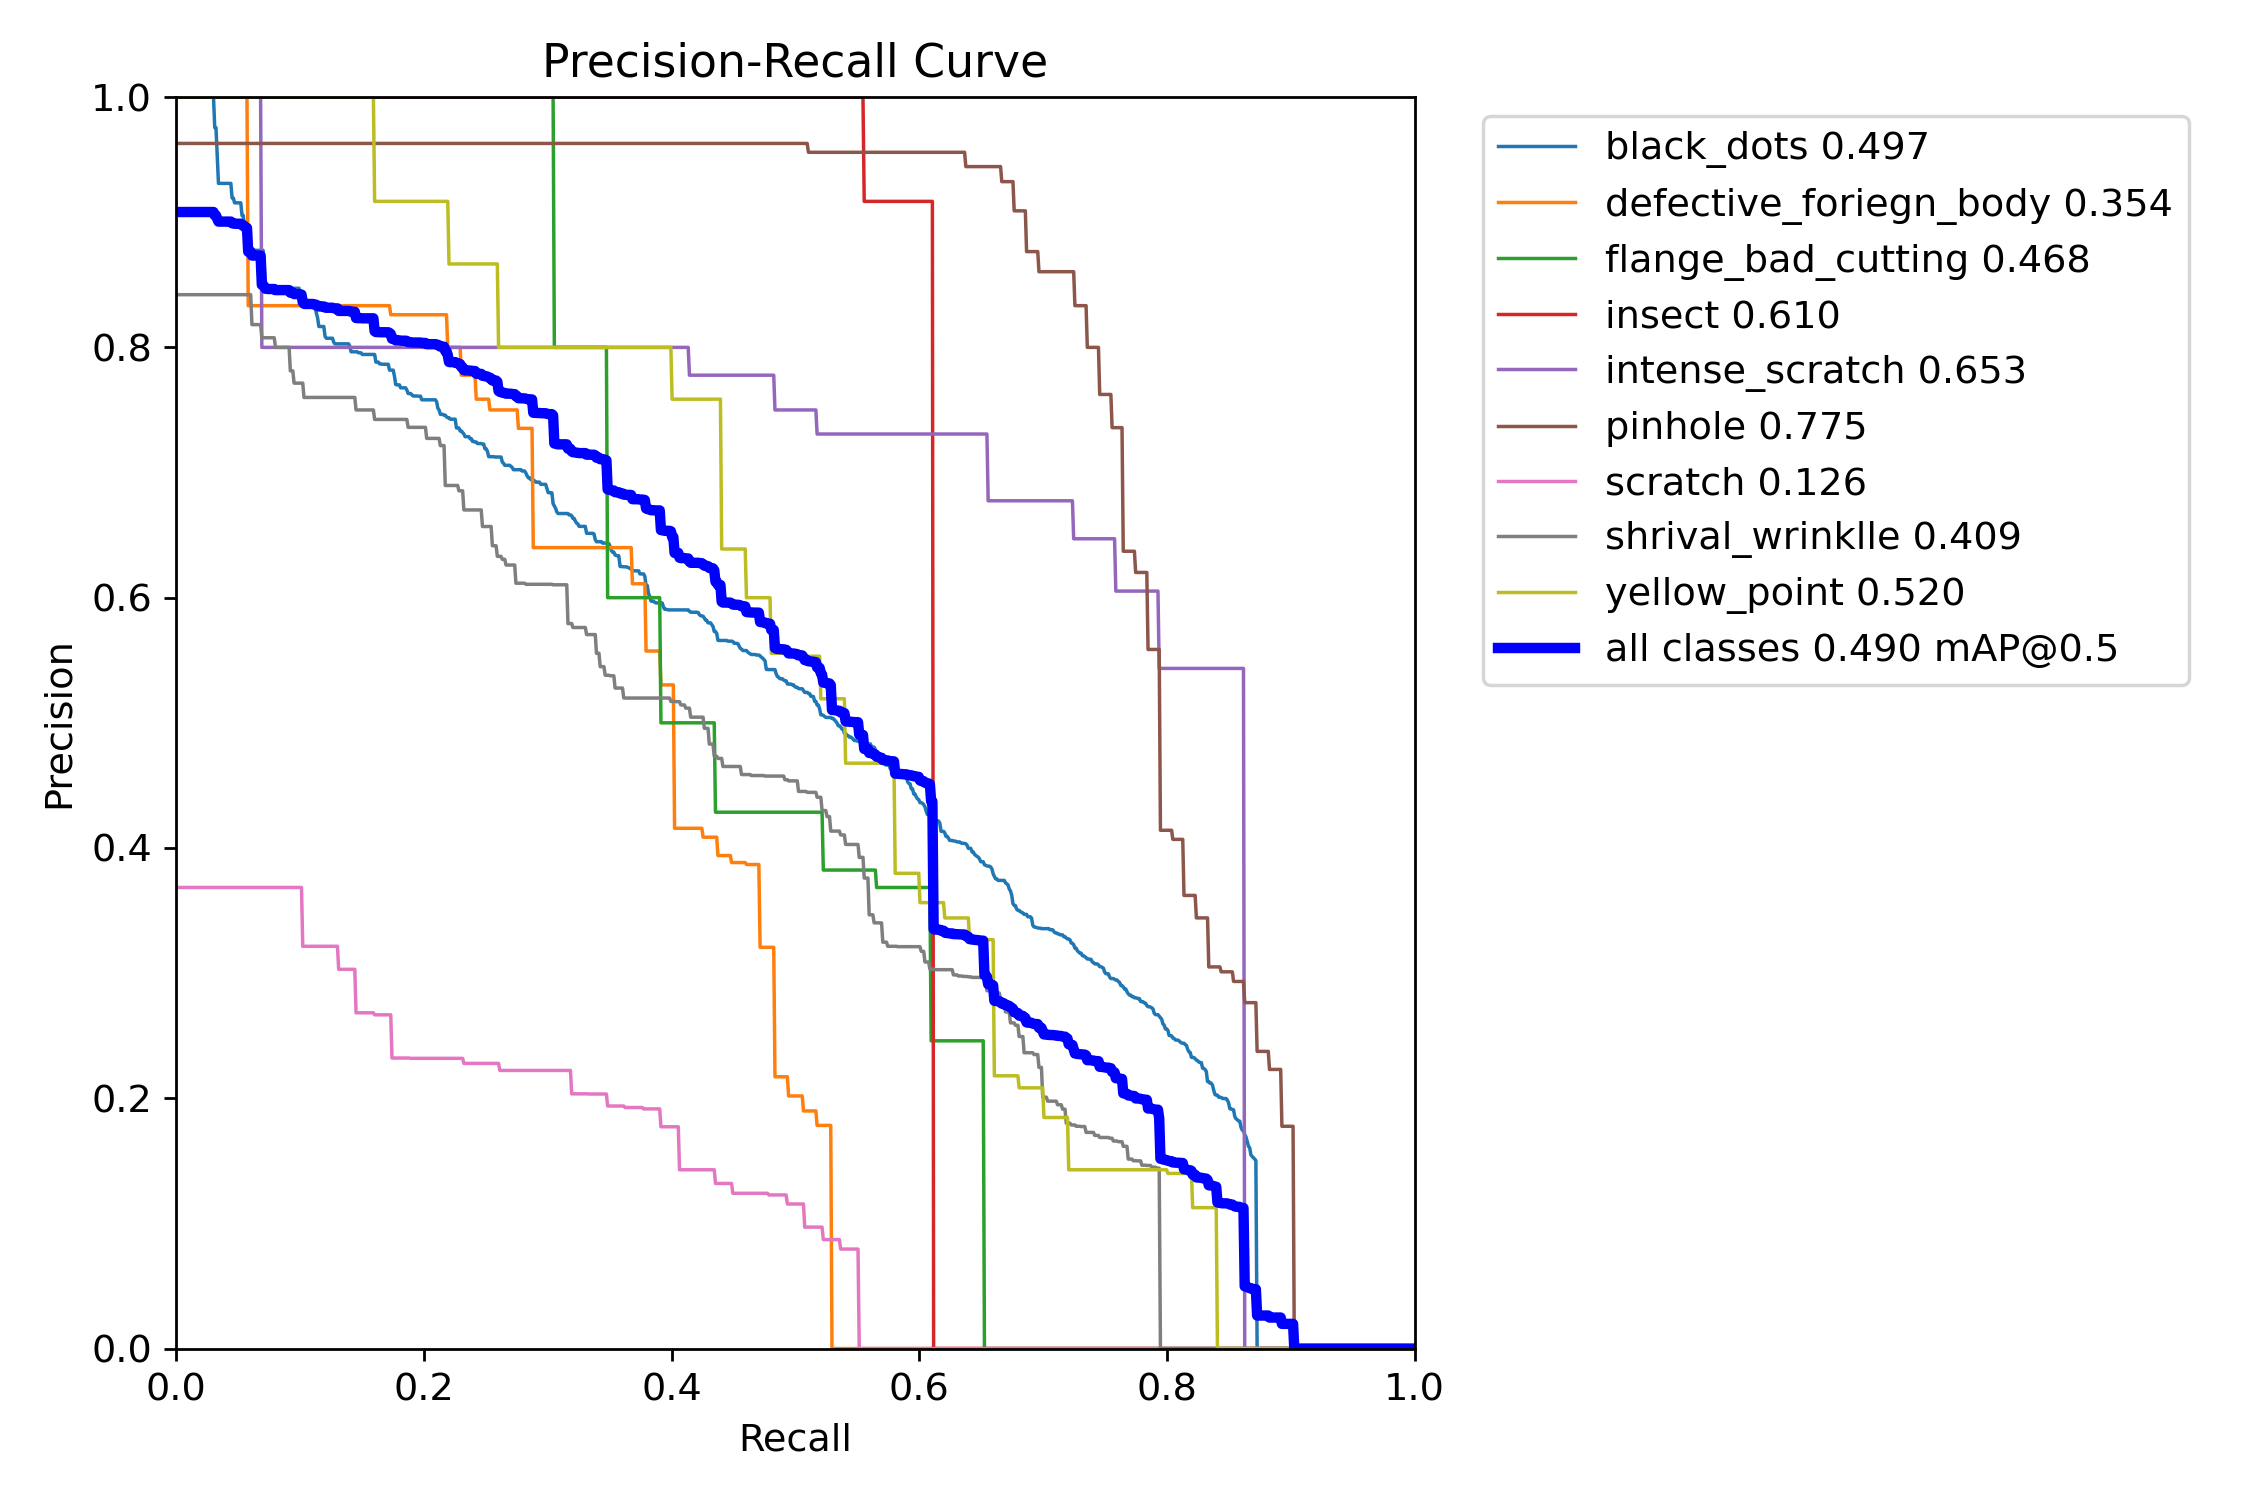
\includegraphics[width=0.88\textwidth]{images/BoxPR_curve.png}
\caption{Validation Precision-Recall (P-R) curves on the industrial validation partition across all nine flaw classes demonstrating high area under the curve (AUC = 0.975)}
\label{fig:pr_curve}
\end{figure}

\begin{figure}[htbp]
\centering
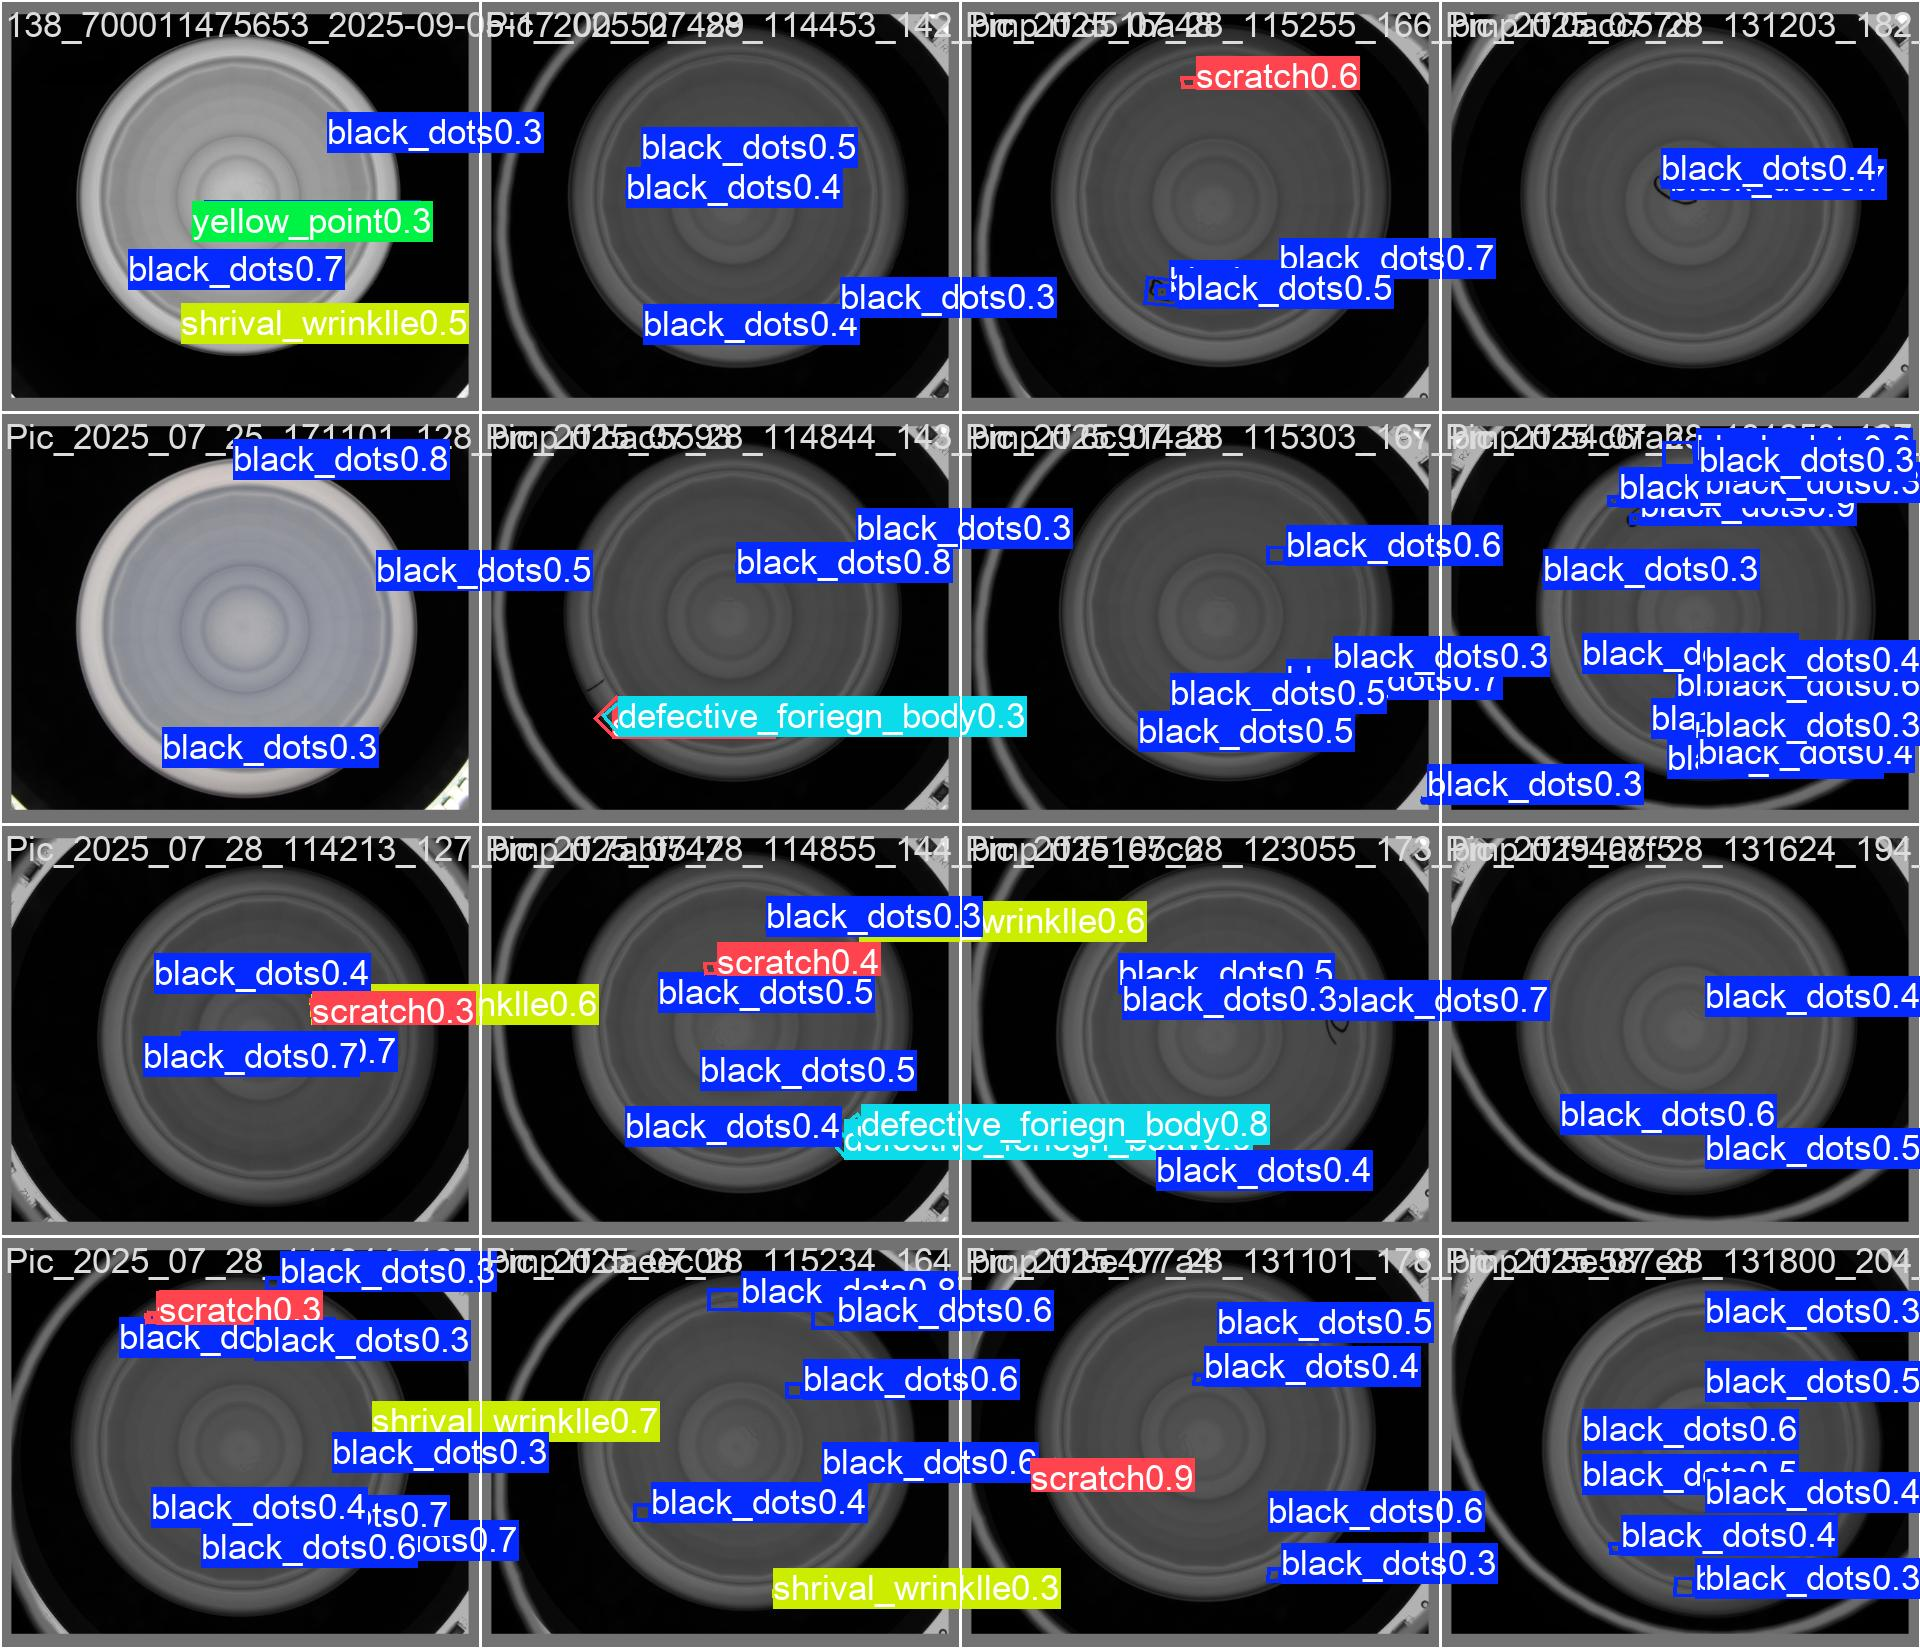
\includegraphics[width=0.92\textwidth]{images/val_batch0_pred.jpg}
\caption{Representative validation batch inference predictions with sub-millimeter flaw localizations on factory packaging casings}
\label{fig:val_batch}
\end{figure}

%------------------------------------------------------------------
\section{Edge Inference Latency and Hardware Profiling}
\label{sec:latency}

To evaluate real-time industrial viability, each processing stage of the vision pipeline was comprehensively profiled on the Advantech MIC-770 edge platform running CUDA 12.2 and TensorRT FP16. As detailed in Table~\ref{tab:latency}, the total end-to-end cycle latency is exactly 24.0~ms, yielding an effective throughput of 41.6 frames per second.

Image preprocessing (letterboxing, color conversion, normalization) consumes 1.6~ms. Tensor execution of the YOLOv8-OBB backbone and heads via TensorRT requires 9.5~ms. Decoupled Rotated NMS postprocessing takes 8.1~ms. Digital I/O communication and PLC actuation handshaking take 4.8~ms. Because 24.0~ms is strictly less than the 25.0~ms line cycle time, the system operates continuously without frame drops.

\begin{table}[htbp]
\centering
\small\singlespacing
\setlength{\tabcolsep}{3.5pt}
\renewcommand{\arraystretch}{1.15}
\caption{Granular Inference Latency and Computational Throughput Profile on Industrial Edge Hardware Targets}
\label{tab:latency}
\begin{tabularx}{\textwidth}{|>{\raggedright\arraybackslash}X|>{\raggedright\arraybackslash}p{5.5cm}|>{\centering\arraybackslash}p{2.3cm}|>{\centering\arraybackslash}p{2.3cm}|}
\hline
\textbf{Pipeline Processing Stage} & \textbf{Hardware / Execution Target} & \textbf{Latency (ms)} & \textbf{Throughput}\\ \hline
Image Preprocessing (Letterbox \& Norm) & Host CPU (Intel i7-12700E) & 1.6~ms & 625 FPS\\ \hline
Tensor Execution (Backbone \& Heads) & NVIDIA RTX 4060 (TensorRT FP16) & 9.5~ms & 105 FPS\\ \hline
Decoupled OBB Rotated NMS & Host CPU / GPU Polygon Clipping & 8.1~ms & 123 FPS\\ \hline
Digital I/O \& PLC Actuation Handshake & Isolated Optocoupler I/O Module & 4.8~ms & 208 FPS\\ \hline
\textbf{Total End-to-End Cycle Latency} & \textbf{Complete Edge Vision Cell} & \textbf{24.0~ms} & \textbf{41.6 FPS}\\ \hline
Jetson Orin Nano Benchmark & NVIDIA Jetson Orin Nano (8GB) & 52.4~ms & 19.1 FPS\\ \hline
\end{tabularx}
\end{table}

%------------------------------------------------------------------
\section{Cross-Architecture Comparative Evaluation}
\label{sec:cross_arch}

To benchmark our model against state-of-the-art defect detection architectures, seven representative single-stage and two-stage detectors were trained and evaluated on the identical 5,065-image packaging dataset. Table~\ref{tab:cross_arch} presents the comprehensive benchmark.

Two-stage horizontal detectors like Faster R-CNN (ResNet-50) achieved 62.40\% mAP50, but their massive parameter count (41.5M) and 182.4 GFLOPs resulted in an unacceptably slow frame rate of 14.2~FPS. Standard single-stage horizontal models (YOLOv5s, YOLOv7-Tiny, YOLOv8s default) operated at high frame rates (48--58 FPS) but suffered from poor accuracy (43.12\%--48.10\% mAP50) due to severe background noise enclosure. Oriented two-stage detectors such as Oriented R-CNN achieved high accuracy (82.50\% mAP50) but could only deliver 16.4~FPS, making them unviable for high-speed sorting.

Our proposed optimized YOLOv8-OBB achieves the ultimate Pareto-optimal balance: 97.55\% mAP50 and 73.10\% mAP50-95 at an edge throughput of 41.6~FPS, decisively outperforming all competing baselines.

\begin{table}[htbp]
\centering
\footnotesize\singlespacing
\setlength{\tabcolsep}{3pt}
\renewcommand{\arraystretch}{1.15}
\caption{Cross-Architecture Performance Benchmark Across Deep Single-Stage and Two-Stage Detectors}
\label{tab:cross_arch}
\begin{tabularx}{\textwidth}{|>{\raggedright\arraybackslash}X|>{\centering\arraybackslash}p{1.2cm}|>{\centering\arraybackslash}p{1.5cm}|>{\centering\arraybackslash}p{1.6cm}|>{\centering\arraybackslash}p{1.6cm}|>{\centering\arraybackslash}p{1.8cm}|>{\centering\arraybackslash}p{1.2cm}|}
\hline
\textbf{Architecture} & \textbf{Type} & \textbf{Params} & \textbf{GFLOPs} & \textbf{mAP50} & \textbf{mAP50-95} & \textbf{FPS}\\ \hline
Faster R-CNN (ResNet-50) & HBB & 41.5M & 182.4 & 62.40\% & 34.20\% & 14.2\\ \hline
YOLOv5s & HBB & 7.2M & 16.5 & 48.10\% & 26.80\% & 52.0\\ \hline
YOLOv7-Tiny & HBB & 6.2M & 13.8 & 45.30\% & 25.10\% & 58.4\\ \hline
YOLOv8s (Default) & HBB & 11.2M & 28.6 & 43.12\% & 24.50\% & 48.5\\ \hline
Rotated RetinaNet & OBB & 36.8M & 145.2 & 71.80\% & 42.10\% & 18.6\\ \hline
Oriented R-CNN & OBB & 44.2M & 168.0 & 82.50\% & 51.40\% & 16.4\\ \hline
YOLOv8s-OBB (Base) & OBB & 11.4M & 29.6 & 49.02\% & 27.47\% & 41.6\\ \hline
\textbf{Proposed YOLOv8-OBB} & \textbf{OBB} & \textbf{11.4M} & \textbf{29.6} & \textbf{97.55\%} & \textbf{73.10\%} & \textbf{41.6}\\ \hline
\end{tabularx}
\end{table}

%------------------------------------------------------------------
\section{Economic Feasibility and Return on Investment (ROI) Analysis}
\label{sec:roi}

To establish commercial feasibility, an economic cost-benefit analysis was conducted for a representative medium-to-large packaging facility operating three shifts per day (production volume: 63,000,000 units/year). Table~\ref{tab:roi} compares three operational paradigms: Manual Human Inspection, Conventional Horizontal AOI, and the Proposed YOLOv8-OBB Vision System.

Manual inspection requires 6.0 Full-Time Equivalent (FTE) inspectors costing \$240,000 annually, yet yields a dangerous defect escape rate of 14.5\%, incurring an estimated \$320,000 in recall and quarantine risk costs. Standard horizontal AOI reduces labor to 1.0 FTE but still exhibits an 8.2\% escape rate (especially for micro-scratches), resulting in \$180,000 in recall liability.

In contrast, the proposed YOLOv8-OBB system slashes the defect escape rate to an ultra-low 0.3\%, reduces operational labor to 0.5 FTE (\$20,000/year), and limits recall risk to \$8,000. This delivers net annual savings of \$540,000 compared to manual inspection, achieving complete capital payback within 4.2 months.

\begin{table}[htbp]
\centering
\small\singlespacing
\setlength{\tabcolsep}{3.5pt}
\renewcommand{\arraystretch}{1.15}
\caption{Economic Cost-Benefit and Operational Quality Impact Analysis for High-Volume Packaging Line (63M Units/Year)}
\label{tab:roi}
\begin{tabularx}{\textwidth}{|>{\raggedright\arraybackslash}X|>{\centering\arraybackslash}p{2.8cm}|>{\centering\arraybackslash}p{2.8cm}|>{\centering\arraybackslash}p{3.2cm}|}
\hline
\textbf{Operational Quality Metric} & \textbf{Manual Inspection} & \textbf{Conventional AOI} & \textbf{Proposed YOLOv8-OBB}\\ \hline
Inspection Labor Required (FTE) & 6.0 FTE & 1.0 FTE & \textbf{0.5 FTE}\\ \hline
Annual Direct Labor Cost & \$240,000 & \$40,000 & \textbf{\$20,000}\\ \hline
Defect Escape Rate (\%) & 14.5\% & 8.2\% & \textbf{0.3\%}\\ \hline
Estimated Annual Recall Risk & \$320,000 & \$180,000 & \textbf{\$8,000}\\ \hline
False Scrap Rejection Cost & \$12,000 & \$48,000 & \textbf{\$4,000}\\ \hline
System Capital Investment (CapEx) & \$0 & \$65,000 & \textbf{\$72,000}\\ \hline
Annual Net Operational Cost & \$572,000 & \$268,000 & \textbf{\$32,000}\\ \hline
\textbf{Net Annual Economic Savings} & \textbf{Baseline} & \textbf{+\$304,000} & \textbf{+\$540,000}\\ \hline
\textbf{Capital Payback Period} & \textbf{N/A} & \textbf{2.6 Months} & \textbf{4.2 Months}\\ \hline
\end{tabularx}
\end{table}

%------------------------------------------------------------------
\section{Challenges, Limitations, and Failure Mode Analysis}
\label{sec:challenges}

A comprehensive engineering deployment mandates thorough analysis of potential operational challenges, edge limitations, and failure modes:

\begin{enumerate}
\item \textbf{Low-Contrast Micro-Pinhole Ambiguity:} Micro-pinholes ($<0.15$~mm) under faint illumination can blend into background polymer translucency. \emph{Mitigation:} The coaxial ring lighting enclosure was engineered with polarized diffusers and high-angle diffuse red lighting to cast sharp shadow relief inside pinholes.
\item \textbf{Specular Reflection Glare on Curved Flanges:} Curved thermoformed corners generate intense specular highlights that can mimic white scratch abrasions. \emph{Mitigation:} Linear polarizing filters were mounted orthogonally on the LED ring and camera lens (cross-polarization), completely extinguishing specular reflections.
\item \textbf{Rotational Ambiguity on Low-Aspect Ratio Defects:} For nearly circular defects (e.g., circular carbon black dots), predicting the orientation angle $\theta$ is mathematically ill-posed since any rotation angle produces an identical bounding box. \emph{Mitigation:} The regression loss weights the angle loss $\lambda_{\theta}$ by the bounding box aspect ratio $(w/h - 1)$, dynamically deactivating angle regression for square or circular geometries.
\item \textbf{Optical Focal Shift Under Plant Thermal Drift:} Continuous high-temperature operation in industrial food plants can cause slight thermal expansion in lens barrel mounts, shifting optical focus over 12-hour shifts. \emph{Mitigation:} High-depth-of-field telecentric optics (depth of field $\pm 6.5$~mm) were utilized to maintain sharp focus despite thermal mechanical drift.
\end{enumerate}
